 \documentclass{article}
\usepackage[utf8]{inputenc}
\usepackage[top=3cm, bottom=3cm, left=3cm,right=3cm]{geometry}
%\usepackage[numbers,round]{natbib}
\usepackage{natbib}
\setcitestyle{aysep={}} 
\usepackage{graphicx}
\usepackage{color}
\usepackage{amsmath}
\usepackage{setspace}
\usepackage{amsmath}
\usepackage{mathtools}
\usepackage{bbm}
\usepackage{float}
\usepackage{hyperref}
\usepackage[super]{nth}

\parindent0cm
\parskip0.5cm
\hyphenpenalty=10000
\pretolerance=10000
\usepackage{lineno}
\linenumbers

\makeatletter
\newcommand{\customlabel}[2]{
\protected@write \@auxout {}{\string \newlabel {#1}{{#2}{}}}}
\makeatother

%\renewcommand\footnote[2][]{\relax}

\begin{document}
{\Large The epidemic lambda-coalescent model}

%Journal target:  Journal of Theoretical Biology? Theoretical Population Biology?

\vspace*{2cm}
Xavier Didelot$^{1,2,*}$, Ian Roberts$^{2}$, ...

\vspace*{2cm}
$^1$ School of Life Sciences, University of Warwick, United Kingdom\\\\
$^2$ Department of Statistics, University of Warwick, United Kingdom\\\\
$^*$ Corresponding author. Tel: 0044 (0)2476 572827. Email: \verb+xavier.didelot@gmail.com+

\vspace*{2cm}
Running title: Epidemic lambda-coalescent

\vspace*{2cm}
Keywords: lambda-coalescent model; pathogen phylogenetics; multiple mergers; offspring distribution

%\newpage
%\section*{Abstract}
%TODO

\newpage
\section{Introduction}

Superspreading in infectious disease epidemiology \citep{Lloyd-Smith2005}.
For example SARS-CoV-2 superspreading \citep{Wang2020,lemieuxPhylogeneticAnalysisSARSCoV22021,gomez-carballaSuperspreadingEmergenceCOVID192021}.
Coalescent model \citep{Kingman1982,Kingman1982a}.
Work by Li and Fraser \citep{Li2017,Fraser2017}.
Lambda-coalescent models \citep{pitmanCoalescentsMultipleCollisions1999,sagitovGeneralCoalescentAsynchronous1999,donnellyParticleRepresentationsMeasureValued1999}. 
Beta-coalescent \citep{schweinsbergCoalescentProcessesObtained2003} is a specific type of Lambda-coalescent. 
Was used in \citep{Hoscheit2019} and \citep{Menardo2021}. 
David's paper \citep{Helekal2024}.

\section{Coalescence probabilities}

\subsection{General case}

Discrete time $t$. Non-overlapping generations of infected individuals. At time $t$ there are $N_t$ infected individuals. Each of them creates a number $k_{t,i}$ of secondary infections at time $t+1$, following the offspring distribution $\alpha_t(k)$. The mean of this distribution is the basic reproduction number $R_t$ and the variance is $v_t$. We have:

\begin{equation}
N_{t+1}=\sum_{i=1}^{N_t} k_{t,i}
\label{eq:summation}
\end{equation}

Let $p_{n,t}$ be the probability that $n$ individuals at time $t+1$ have the same infector at time $t$.

\subsection{Poisson case}

Here the offspring distribution is Poisson($R_t$).

The probability of coalescence for two lines is:
\begin{equation}
p_{2,t}=\frac{1}{N_t}
\end{equation}

The probability of coalescence for $n$ lines is:

\begin{equation}
p_{n,t}=\frac{1}{N_t^{n-1}}
\end{equation}

\subsection{NegBin case}

Here the offspring distribution is Negative-Binomial with mean $R_t$ and variance $v_t$.
The parameters of this distribution are 
$r=R_t^2/(v_t-R_t)$ and $p=R_t/v_t$.

The probability of coalescence for two lines is:

\begin{equation}
p_{2,t}=\frac{r+1}{N_t r+1}
\end{equation}

The probability of coalescence for $n$ lines is:

\begin{equation}
p_{n,t}=\frac{\prod_{i=1}^{n-1}r+i}{\prod_{i=1}^{n-1}N_t r+i}
\end{equation}

\subsection{Example}

See Figure \ref{fig:probs}.

\begin{figure}[t!]
\begin{center}
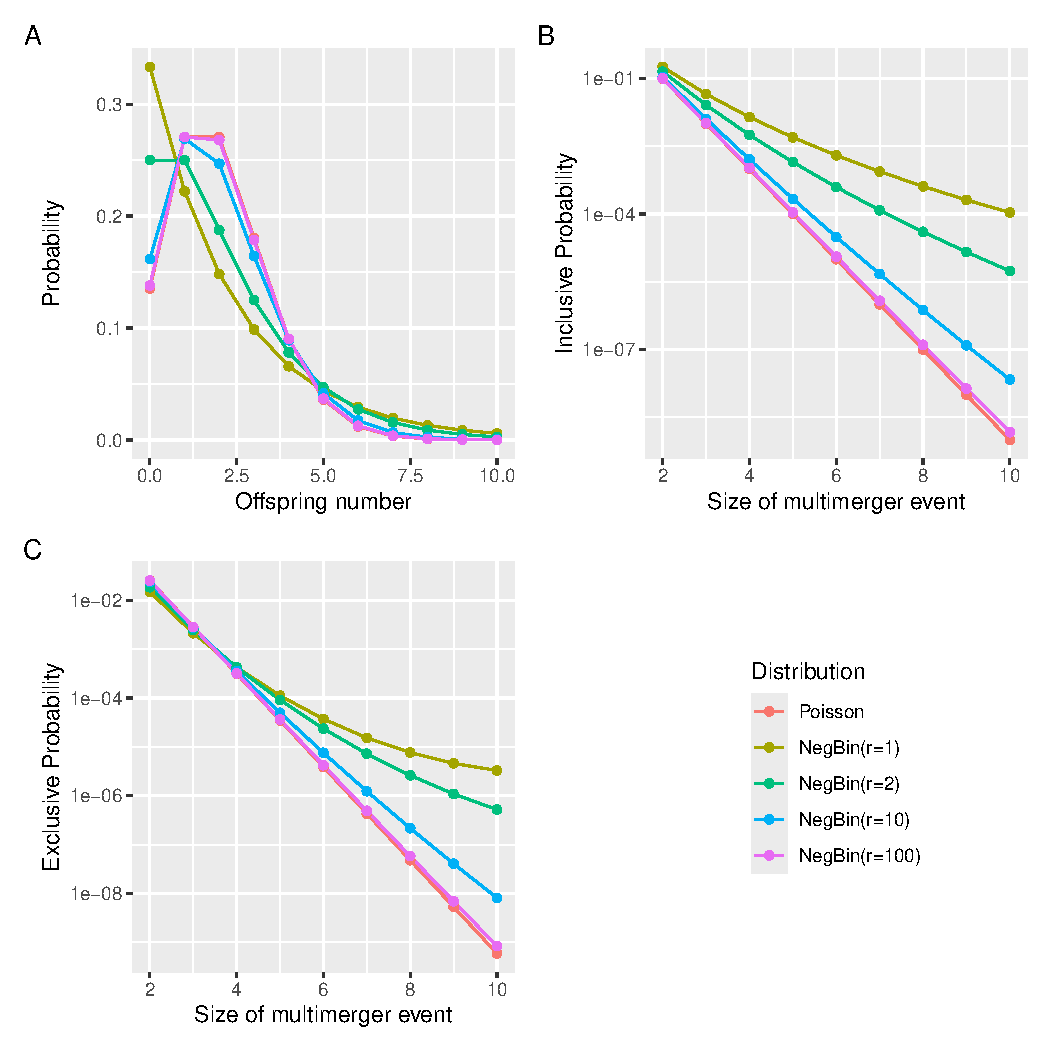
\includegraphics[width=15cm]{../run/figure.pdf}
\end{center}
\caption{(A) Offspring distribution. (B) Probability of coalescence.
\label{fig:probs}}
\end{figure}

\section{Implementation}

We implemented the analytical methods described in this paper in a 
new R package entitled \emph{EpiLambda} which is available
at \url{https://github.com/xavierdidelot/EpiLambda} for R version 3.5 or later. 
All code and data needed to replicate the results are included in the ``run'' directory of the \emph{EpiLambda} repository.

\section{Discussion}

\section*{Acknowledgements}

We acknowledge funding from the National Institute for Health Research (NIHR) Health Protection Research Unit in Genomics and Enabling Data.

\newpage
\bibliographystyle{elsarticle-harv}
\bibliography{biblio,/Users/u1775021/all.bib}

\end{document}

